\documentclass[tikz,border=8pt]{standalone}
\usepackage{ctex}
\usepackage{amsmath,amssymb,bm}
\usetikzlibrary{arrows.meta,calc,angles,quotes,decorations.pathmorphing,patterns,positioning,3d}
\definecolor{ink}{RGB}{30,43,58}
\definecolor{blue}{RGB}{37,91,166}
\definecolor{orange}{RGB}{219,113,25}
\definecolor{green}{RGB}{39,139,94}
\definecolor{red}{RGB}{192,52,52}
\tikzset{
 line cap=round,line join=round,
 body/.style={draw=ink,very thick},
 axis/.style={-{Latex[length=2.5mm]},draw=ink,very thick},
 vec/.style={-{Latex[length=2.5mm]},draw=blue,very thick},
 force/.style={-{Latex[length=2.5mm]},draw=red,very thick},
 guide/.style={draw=ink!45,dashed},
 dim/.style={{Latex[length=2mm]}-{Latex[length=2mm]},draw=ink!75},
 current/.style={-{Latex[length=2.5mm]},draw=orange,very thick}
}

\tikzset{mass/.style={circle,draw,fill=white,minimum size=7mm},curve/.style={very thick,blue},rope/.style={very thick,blue},ray/.style={very thick,blue,-{Latex}},impulse/.style={very thick,orange,-{Latex}},resistor/.style={thick,decorate,decoration={zigzag,segment length=3mm,amplitude=1mm}}}
\begin{document}
% 1 question-01
\begin{tikzpicture}[scale=1]
  % 左侧放大起点附近，避免 $r_1/r_0=e^{2\pi/\sqrt3}$ 使切向关系不可读。
  \begin{scope}[shift={(-4.0,-.45)},scale=.78]
    \draw[rounded corners=3pt,draw=ink!35] (-.45,-1.35) rectangle (3.35,3.15);
    \draw[axis] (-.15,0)--(2.95,0) node[right] {$\bm e_r$};
    \draw[axis] (0,-.25)--(0,2.65) node[above] {$\bm e_\theta$};
    \draw[very thick,blue,domain=0:68,samples=90,smooth,variable=\t]
      plot ({exp(\t/99.24)*cos(\t)},{exp(\t/99.24)*sin(\t)});
    \coordinate (P) at (1,0);
    \fill[orange] (P) circle(2.4pt) node[below right] {$P:\ \theta=0,\ r_0=1\ \mathrm m$};
    \draw[force] (P)--++(1.0,1.732) node[above right] {$\bm v_0$};
    \coordinate (R) at (2.35,0);
    \coordinate (T) at (2,1.732);
    \pic[draw=ink,"$60^\circ$",angle radius=7mm,angle eccentricity=1.28]
      {angle=R--P--T};
  \end{scope}

  % 右侧用同一缩尺绘出完整一周，保留螺线的真实径向比。
  \coordinate (O) at (0,0);
  \draw[axis] (-1.0,0)--(5.25,0) node[right] {$x$};
  \draw[axis] (0,-2.15)--(0,1.15) node[above] {$y$};
  \draw[very thick,blue,domain=0:360,samples=240,smooth,variable=\t]
    plot ({.12*exp(\t/99.24)*cos(\t)},{.12*exp(\t/99.24)*sin(\t)});
  \fill (O) circle(2pt) node[above left] {$O$};
  \fill[orange] (.12,0) circle(2.2pt);
  \fill ({.12*exp(360/99.24)},0) circle(2.2pt)
    node[above left] {$\theta=2\pi,\ r_1=e^{2\pi/\sqrt3}r_0$};
  \node[ink!75] at (2.45,-2.28) {完整一周（全图统一缩尺）};
  \node[align=center] at (2.75,1.32)
    {等角螺线 $r=e^{\theta/\sqrt3}$\\整体可绕过 $O$ 的竖直轴转动};
\end{tikzpicture}

% 2 solution-01
\begin{tikzpicture}[x=1cm,y=1cm,font=\small]

\coordinate(P)at(0,0);\draw[axis](-1,0)--(3.3,0)node[right]{$\boldsymbol e_r$};\draw[axis](0,-1.4)--(0,3)node[above]{$\boldsymbol e_\theta$};
\draw[vec,orange](P)--(1,1.732)node[above]{$\boldsymbol v_{\rm rel}$};
\draw[vec,red](1,1.732)--(1,1.032)node[right]{$\omega r\boldsymbol e_\theta$};\draw[vec,green](P)--(1,1.032)node[left]{$\boldsymbol v_{\rm abs}$};
\draw(.7,0)arc(0:60:.7)node[midway,right]{$60^\circ$};
\node[align=left,anchor=west]at(4,.7){$r=r_0e^{\theta/\sqrt3}$\\$\mathrm ds=2\mathrm dr$\\$\boldsymbol v_{\rm abs}=\boldsymbol v_{\rm rel}+\omega r\boldsymbol e_\theta$\\$\omega<0$时方位分量相减};
\end{tikzpicture}

% 3 question-02
\begin{tikzpicture}[scale=.8,font=\small]

\draw[body](-1,0)--(0,0)--(0,-1.5);\draw[body](10,-1.5)--(10,0)--(12,0);
\draw[body,orange](0,1)--(3,1);\draw[body](0,1)circle(1);\draw[body](3,1)circle(1);
\draw[dim](0,2.4)--(3,2.4)node[midway,above]{$3r$};\draw[dim](0,-2)--(10,-2)node[midway,below]{$10r$};
\draw[dashed,blue] plot coordinates {(3.000000,1.000000) (3.065657,0.999986) (3.131313,0.999945) (3.196970,0.999877) (3.262626,0.999781) (3.328283,0.999658) (3.393939,0.999508) (3.459596,0.999330) (3.525252,0.999125) (3.590909,0.998893) (3.656566,0.998633) (3.722222,0.998346) (3.787879,0.998032) (3.853535,0.997690) (3.919192,0.997321) (3.984848,0.996924) (4.050505,0.996501) (4.116161,0.996049) (4.181818,0.995571) (4.247475,0.995065) (4.313131,0.994532) (4.378788,0.993972) (4.444444,0.993384) (4.510101,0.992769) (4.575757,0.992126) (4.641414,0.991457) (4.707070,0.990759) (4.772727,0.990035) (4.838383,0.989283) (4.904040,0.988504) (4.969697,0.987697) (5.035353,0.986864) (5.101010,0.986002) (5.166666,0.985114) (5.232323,0.984198) (5.297979,0.983255) (5.363636,0.982284) (5.429292,0.981286) (5.494949,0.980261) (5.560606,0.979209) (5.626262,0.978129) (5.691919,0.977021) (5.757575,0.975887) (5.823232,0.974725) (5.888888,0.973536) (5.954545,0.972319) (6.020201,0.971075) (6.085858,0.969804) (6.151515,0.968505) (6.217171,0.967179) (6.282828,0.965826) (6.348484,0.964445) (6.414141,0.963038) (6.479797,0.961602) (6.545454,0.960140) (6.611110,0.958650) (6.676767,0.957132) (6.742424,0.955588) (6.808080,0.954016) (6.873737,0.952416) (6.939393,0.950790) (7.005050,0.949136) (7.070706,0.947454) (7.136363,0.945746) (7.202019,0.944010) (7.267676,0.942246) (7.333333,0.940455) (7.398989,0.938637) (7.464646,0.936792) (7.530302,0.934919) (7.595959,0.933019) (7.661615,0.931092) (7.727272,0.929137) (7.792928,0.927155) (7.858585,0.925146) (7.924241,0.923109) (7.989898,0.921045) (8.055555,0.918953) (8.121211,0.916834) (8.186868,0.914688) (8.252524,0.912515) (8.318181,0.910314) (8.383837,0.908086) (8.449494,0.905830) (8.515150,0.903548) (8.580807,0.901237) (8.646464,0.898900) (8.712120,0.896535) (8.777777,0.894143) (8.843433,0.891723) (8.909090,0.889277) (8.974746,0.886802) (9.040403,0.884301) (9.106059,0.881772) (9.171716,0.879216) (9.237373,0.876632) (9.303029,0.874021) (9.368686,0.871383) (9.434342,0.868718) (9.499999,0.866025)};
\draw[vec](4,2)--(6.5,2)node[above]{$v$};\node at(6,-3){虚线为前轮轮心碰前平抛轨迹，半径均为$r$};
\end{tikzpicture}

% 4 solution-02
\begin{tikzpicture}[x=1cm,y=1cm,font=\small]

\begin{scope}[shift={(-2.1,.2)}]\fill[ink!8](0,-1.3)rectangle(2,0);\draw[body](0,-1.3)--(0,0)--(2,0);
\draw[body,orange](-3.5,.866)--(-.5,.866);\draw[body](-.5,.866)circle(1);\draw[body](-3.5,.866)circle(1);
\draw[force](-.5,.866)--(-1.1,1.906)node[above]{$p\boldsymbol n$};\draw[force](-.5,.866)--(.54,1.466)node[right]{$j\boldsymbol t$};
\draw[very thick,green] plot coordinates {(-3.500001,0.866025) (-3.481881,0.858461) (-3.463582,0.850896) (-3.445102,0.843332) (-3.426443,0.835769) (-3.407604,0.828211) (-3.388585,0.820659) (-3.369387,0.813115) (-3.350010,0.805581) (-3.330453,0.798059) (-3.310718,0.790552) (-3.290803,0.783060) (-3.270711,0.775586) (-3.250439,0.768132) (-3.229990,0.760700) (-3.209363,0.753292) (-3.188559,0.745909) (-3.167577,0.738554) (-3.146419,0.731229) (-3.125084,0.723936) (-3.103574,0.716675) (-3.081887,0.709451) (-3.060026,0.702263) (-3.037990,0.695115) (-3.015780,0.688008) (-2.993396,0.680944) (-2.970839,0.673925) (-2.948109,0.666953) (-2.925207,0.660029) (-2.902134,0.653156) (-2.878890,0.646336) (-2.855476,0.639570) (-2.831892,0.632860) (-2.808139,0.626208) (-2.784218,0.619617) (-2.760129,0.613087) (-2.735874,0.606620) (-2.711453,0.600219) (-2.686866,0.593885) (-2.662114,0.587620) (-2.637199,0.581427) (-2.612122,0.575305) (-2.586882,0.569258) (-2.561481,0.563287) (-2.535919,0.557395) (-2.510198,0.551581) (-2.484319,0.545850) (-2.458282,0.540201) (-2.432089,0.534637) (-2.405740,0.529160) (-2.379237,0.523771) (-2.352580,0.518472) (-2.325770,0.513265) (-2.298809,0.508151) (-2.271697,0.503132) (-2.244437,0.498210) (-2.217028,0.493385) (-2.189472,0.488661) (-2.161769,0.484038) (-2.133923,0.479518) (-2.105932,0.475103) (-2.077799,0.470794) (-2.049525,0.466592) (-2.021111,0.462500) (-1.992558,0.458519) (-1.963868,0.454650) (-1.935042,0.450895) (-1.906080,0.447255) (-1.876985,0.443732) (-1.847758,0.440327) (-1.818400,0.437042) (-1.788912,0.433877) (-1.759296,0.430836) (-1.729554,0.427918) (-1.699686,0.425126) (-1.669694,0.422460) (-1.639579,0.419922) (-1.609344,0.417513) (-1.578988,0.415235) (-1.548515,0.413090) (-1.517925,0.411077) (-1.487220,0.409199) (-1.456401,0.407456) (-1.425470,0.405851) (-1.394428,0.404383) (-1.363278,0.403056) (-1.332020,0.401868) (-1.300656,0.400823) (-1.269188,0.399920) (-1.237618,0.399162) (-1.205946,0.398548) (-1.174175,0.398081) (-1.142306,0.397761) (-1.110342,0.397590) (-1.078283,0.397568) (-1.046131,0.397697) (-1.013888,0.397976) (-0.981556,0.398409) (-0.949136,0.398995) (-0.916631,0.399735)};
\fill (-0.916631,0.399735) circle(2pt) node[below] {$B_{
m touch}$};
\end{scope}\begin{scope}[shift={(2.8,-.6)}]\draw[axis](0,0)--(4.5,0)node[right]{$p$};\draw[axis](0,-1.6)--(0,1.6)node[above]{$v_t$};\draw[very thick,blue](0,-1.2)--(1,0)--(4,.422);\fill(1,0)circle(2pt)node[above]{$p_s$};\node[above]at(.5,-.6){$+\mu$};\node[below]at(2.5,.2){$-\mu$};\node at(2,-2.2){静摩擦不足，随后反向滑动};\end{scope}
\end{tikzpicture}

% 5 question-03
\begin{tikzpicture}[x=1cm,y=1cm,font=\small]
\draw[axis](0,0)--(6.5,0)node[right]{$V/V_A$};\draw[axis](0,0)--(0,4.5)node[above]{$p/p_A$};\draw[very thick,orange,-{Latex}] plot coordinates {(2.000000,2.000000) (2.366432,2.366432)};
\draw[very thick,red,-{Latex}] plot coordinates {(2.366432,2.366432) (2.397963,2.322984) (2.429494,2.280886) (2.461025,2.240078) (2.492556,2.200507) (2.524087,2.162119) (2.555618,2.124865) (2.587149,2.088698) (2.618680,2.053574) (2.650211,2.019450) (2.681742,1.986286) (2.713273,1.954046) (2.744804,1.922692) (2.776335,1.892191) (2.807866,1.862511) (2.839397,1.833619) (2.870928,1.805487) (2.902459,1.778088) (2.933990,1.751393) (2.965521,1.725378) (2.997052,1.700019) (3.028583,1.675292) (3.060114,1.651175) (3.091645,1.627647) (3.123176,1.604688) (3.154707,1.582279) (3.186238,1.560401) (3.217769,1.539036) (3.249300,1.518168) (3.280831,1.497781) (3.312362,1.477858) (3.343893,1.458386) (3.375424,1.439349) (3.406955,1.420734) (3.438486,1.402528) (3.470017,1.384718) (3.501548,1.367293) (3.533079,1.350240) (3.564610,1.333549) (3.596141,1.317208) (3.627672,1.301207) (3.659203,1.285537) (3.690734,1.270188) (3.722265,1.255150) (3.753796,1.240414) (3.785326,1.225973) (3.816857,1.211818) (3.848388,1.197940) (3.879919,1.184333) (3.911450,1.170989) (3.942981,1.157900) (3.974512,1.145060) (4.006043,1.132462) (4.037574,1.120100) (4.069105,1.107968) (4.100636,1.096059) (4.132167,1.084368) (4.163698,1.072889) (4.195229,1.061616) (4.226760,1.050546) (4.258291,1.039671) (4.289822,1.028989) (4.321353,1.018493) (4.352884,1.008179) (4.384415,0.998043) (4.415946,0.988081) (4.447477,0.978287) (4.479008,0.968659) (4.510539,0.959193) (4.542070,0.949883) (4.573601,0.940728) (4.605132,0.931723) (4.636663,0.922864) (4.668194,0.914149) (4.699725,0.905574) (4.731256,0.897137) (4.762787,0.888833) (4.794318,0.880660) (4.825849,0.872614) (4.857380,0.864695) (4.888911,0.856897) (4.920442,0.849219) (4.951973,0.841659) (4.983504,0.834213) (5.015035,0.826879) (5.046566,0.819655) (5.078097,0.812539) (5.109628,0.805528) (5.141159,0.798620) (5.172690,0.791813) (5.204221,0.785105) (5.235752,0.778493) (5.267283,0.771977) (5.298814,0.765553) (5.330345,0.759221) (5.361876,0.752978) (5.393407,0.746822) (5.424938,0.740752) (5.456469,0.734766) (5.488000,0.728863)};
\draw[very thick,green,-{Latex}] plot coordinates {(5.488000,0.728863) (5.452768,0.733572) (5.417535,0.738343) (5.382303,0.743176) (5.347071,0.748073) (5.311838,0.753035) (5.276606,0.758063) (5.241374,0.763159) (5.206141,0.768323) (5.170909,0.773558) (5.135677,0.778865) (5.100444,0.784245) (5.065212,0.789700) (5.029980,0.795232) (4.994747,0.800841) (4.959515,0.806530) (4.924283,0.812301) (4.889051,0.818155) (4.853818,0.824093) (4.818586,0.830119) (4.783354,0.836233) (4.748121,0.842438) (4.712889,0.848736) (4.677657,0.855129) (4.642424,0.861619) (4.607192,0.868208) (4.571960,0.874898) (4.536727,0.881693) (4.501495,0.888594) (4.466263,0.895603) (4.431030,0.902725) (4.395798,0.909960) (4.360566,0.917312) (4.325333,0.924784) (4.290101,0.932379) (4.254869,0.940100) (4.219636,0.947949) (4.184404,0.955931) (4.149172,0.964048) (4.113939,0.972304) (4.078707,0.980703) (4.043475,0.989248) (4.008242,0.997944) (3.973010,1.006793) (3.937778,1.015801) (3.902545,1.024972) (3.867313,1.034310) (3.832081,1.043819) (3.796848,1.053505) (3.761616,1.063373) (3.726384,1.073427) (3.691152,1.083673) (3.655919,1.094116) (3.620687,1.104763) (3.585455,1.115619) (3.550222,1.126690) (3.514990,1.137983) (3.479758,1.149505) (3.444525,1.161263) (3.409293,1.173264) (3.374061,1.185515) (3.338828,1.198025) (3.303596,1.210802) (3.268364,1.223854) (3.233131,1.237191) (3.197899,1.250821) (3.162667,1.264755) (3.127434,1.279004) (3.092202,1.293577) (3.056970,1.308485) (3.021737,1.323742) (2.986505,1.339358) (2.951273,1.355347) (2.916040,1.371723) (2.880808,1.388499) (2.845576,1.405691) (2.810343,1.423314) (2.775111,1.441384) (2.739879,1.459919) (2.704646,1.478936) (2.669414,1.498456) (2.634182,1.518498) (2.598949,1.539083) (2.563717,1.560235) (2.528485,1.581975) (2.493253,1.604330) (2.458020,1.627326) (2.422788,1.650991) (2.387556,1.675354) (2.352323,1.700447) (2.317091,1.726303) (2.281859,1.752957) (2.246626,1.780447) (2.211394,1.808814) (2.176162,1.838099) (2.140929,1.868348) (2.105697,1.899609) (2.070465,1.931933) (2.035232,1.965378) (2.000000,2.000000)};
\fill (2.000000,2.000000) circle(2pt) node[above left] {$A$};
\fill (2.366432,2.366432) circle(2pt) node[above] {$B$};
\fill (5.488000,0.728863) circle(2pt) node[right] {$C$};
\node at(3,-.7){$T_2/T_1=1.4$示例；绿线严格满足$pV=\mathrm{const}$};
\end{tikzpicture}

% 6 solution-03
\begin{tikzpicture}[x=1cm,y=1cm,font=\small]
\draw[axis](0,0)--(6.5,0)node[right]{$V/V_A$};\draw[axis](0,0)--(0,4.5)node[above]{$p/p_A$};\draw[very thick,orange,-{Latex}] plot coordinates {(2.000000,2.000000) (2.366432,2.366432)};
\draw[very thick,red,-{Latex}] plot coordinates {(2.366432,2.366432) (2.397963,2.322984) (2.429494,2.280886) (2.461025,2.240078) (2.492556,2.200507) (2.524087,2.162119) (2.555618,2.124865) (2.587149,2.088698) (2.618680,2.053574) (2.650211,2.019450) (2.681742,1.986286) (2.713273,1.954046) (2.744804,1.922692) (2.776335,1.892191) (2.807866,1.862511) (2.839397,1.833619) (2.870928,1.805487) (2.902459,1.778088) (2.933990,1.751393) (2.965521,1.725378) (2.997052,1.700019) (3.028583,1.675292) (3.060114,1.651175) (3.091645,1.627647) (3.123176,1.604688) (3.154707,1.582279) (3.186238,1.560401) (3.217769,1.539036) (3.249300,1.518168) (3.280831,1.497781) (3.312362,1.477858) (3.343893,1.458386) (3.375424,1.439349) (3.406955,1.420734) (3.438486,1.402528) (3.470017,1.384718) (3.501548,1.367293) (3.533079,1.350240) (3.564610,1.333549) (3.596141,1.317208) (3.627672,1.301207) (3.659203,1.285537) (3.690734,1.270188) (3.722265,1.255150) (3.753796,1.240414) (3.785326,1.225973) (3.816857,1.211818) (3.848388,1.197940) (3.879919,1.184333) (3.911450,1.170989) (3.942981,1.157900) (3.974512,1.145060) (4.006043,1.132462) (4.037574,1.120100) (4.069105,1.107968) (4.100636,1.096059) (4.132167,1.084368) (4.163698,1.072889) (4.195229,1.061616) (4.226760,1.050546) (4.258291,1.039671) (4.289822,1.028989) (4.321353,1.018493) (4.352884,1.008179) (4.384415,0.998043) (4.415946,0.988081) (4.447477,0.978287) (4.479008,0.968659) (4.510539,0.959193) (4.542070,0.949883) (4.573601,0.940728) (4.605132,0.931723) (4.636663,0.922864) (4.668194,0.914149) (4.699725,0.905574) (4.731256,0.897137) (4.762787,0.888833) (4.794318,0.880660) (4.825849,0.872614) (4.857380,0.864695) (4.888911,0.856897) (4.920442,0.849219) (4.951973,0.841659) (4.983504,0.834213) (5.015035,0.826879) (5.046566,0.819655) (5.078097,0.812539) (5.109628,0.805528) (5.141159,0.798620) (5.172690,0.791813) (5.204221,0.785105) (5.235752,0.778493) (5.267283,0.771977) (5.298814,0.765553) (5.330345,0.759221) (5.361876,0.752978) (5.393407,0.746822) (5.424938,0.740752) (5.456469,0.734766) (5.488000,0.728863)};
\draw[very thick,green,-{Latex}] plot coordinates {(5.488000,0.728863) (5.452768,0.733572) (5.417535,0.738343) (5.382303,0.743176) (5.347071,0.748073) (5.311838,0.753035) (5.276606,0.758063) (5.241374,0.763159) (5.206141,0.768323) (5.170909,0.773558) (5.135677,0.778865) (5.100444,0.784245) (5.065212,0.789700) (5.029980,0.795232) (4.994747,0.800841) (4.959515,0.806530) (4.924283,0.812301) (4.889051,0.818155) (4.853818,0.824093) (4.818586,0.830119) (4.783354,0.836233) (4.748121,0.842438) (4.712889,0.848736) (4.677657,0.855129) (4.642424,0.861619) (4.607192,0.868208) (4.571960,0.874898) (4.536727,0.881693) (4.501495,0.888594) (4.466263,0.895603) (4.431030,0.902725) (4.395798,0.909960) (4.360566,0.917312) (4.325333,0.924784) (4.290101,0.932379) (4.254869,0.940100) (4.219636,0.947949) (4.184404,0.955931) (4.149172,0.964048) (4.113939,0.972304) (4.078707,0.980703) (4.043475,0.989248) (4.008242,0.997944) (3.973010,1.006793) (3.937778,1.015801) (3.902545,1.024972) (3.867313,1.034310) (3.832081,1.043819) (3.796848,1.053505) (3.761616,1.063373) (3.726384,1.073427) (3.691152,1.083673) (3.655919,1.094116) (3.620687,1.104763) (3.585455,1.115619) (3.550222,1.126690) (3.514990,1.137983) (3.479758,1.149505) (3.444525,1.161263) (3.409293,1.173264) (3.374061,1.185515) (3.338828,1.198025) (3.303596,1.210802) (3.268364,1.223854) (3.233131,1.237191) (3.197899,1.250821) (3.162667,1.264755) (3.127434,1.279004) (3.092202,1.293577) (3.056970,1.308485) (3.021737,1.323742) (2.986505,1.339358) (2.951273,1.355347) (2.916040,1.371723) (2.880808,1.388499) (2.845576,1.405691) (2.810343,1.423314) (2.775111,1.441384) (2.739879,1.459919) (2.704646,1.478936) (2.669414,1.498456) (2.634182,1.518498) (2.598949,1.539083) (2.563717,1.560235) (2.528485,1.581975) (2.493253,1.604330) (2.458020,1.627326) (2.422788,1.650991) (2.387556,1.675354) (2.352323,1.700447) (2.317091,1.726303) (2.281859,1.752957) (2.246626,1.780447) (2.211394,1.808814) (2.176162,1.838099) (2.140929,1.868348) (2.105697,1.899609) (2.070465,1.931933) (2.035232,1.965378) (2.000000,2.000000)};
\fill (2.000000,2.000000) circle(2pt) node[above left] {$A$};
\fill (2.366432,2.366432) circle(2pt) node[above] {$B$};
\fill (5.488000,0.728863) circle(2pt) node[right] {$C$};
\node at(3,-.7){$T_2/T_1=1.4$示例；绿线严格满足$pV=\mathrm{const}$};
\end{tikzpicture}

% 7 question-04
\begin{tikzpicture}[scale=.9]
  \draw[body] (-3,-3) rectangle (3,3);
  \draw[axis] (-3.5,0)--(3.7,0) node[above right] {$x$};
  \draw[axis] (0,-3.5)--(0,3.7) node[above] {$y$};
  \draw[very thick,orange] (-1.5,-1.5)--(-1.5,1.5)--(1.5,1.5)--(1.5,-1.5);
  \node[orange] at (-2.2,2.25) {$H_1$};
  \begin{scope}[xshift=7.4cm]
    \draw[body] (-3,-3) rectangle (3,3);
    \draw[axis] (-3.5,0)--(3.7,0) node[above right] {$x$};
    \draw[axis] (0,-3.5)--(0,3.7) node[above] {$y$};
    \draw[very thick,blue] (-2.25,-2.25)--(-.75,-2.25)--(-.75,-.75)--(-2.25,-.75)
      --(-2.25,.75)--(-2.25,2.25)--(-.75,2.25)--(-.75,.75)--(.75,.75)
      --(.75,2.25)--(2.25,2.25)--(2.25,.75)--(2.25,-.75)--(.75,-.75)
      --(.75,-2.25)--(2.25,-2.25);
    \node[blue] at (-2.2,2.7) {$H_2$};
  \end{scope}
  \node at (3.7,-4.1) {外框边长均为 $L$，每阶曲线总质量均为 $M$};
\end{tikzpicture}

% 8 solution-04
\begin{tikzpicture}[scale=.93]
  \draw[body] (-3,-3) rectangle (3,3);
  \fill[blue!9] (-3,-3) rectangle (3,3);
  \draw[very thick,orange] (-1.5,-1.5)--(-1.5,1.5)--(1.5,1.5)--(1.5,-1.5);
  \draw[guide] (-3,0)--(3,0); \draw[guide] (0,-3)--(0,3);
  \node[align=left,anchor=west] at (4,-.2)
   {$I_{1x}=\dfrac{5}{144}ML^2,\quad I_{1y}=\dfrac{7}{144}ML^2$\\[7pt]
    $I_{2x}=\dfrac{197}{2880}ML^2,\quad I_{2y}=\dfrac{199}{2880}ML^2$\\[7pt]
    归一化弧长测度趋于均匀面积测度\\[2pt]
    $I_{\infty x}=I_{\infty y}=\dfrac{ML^2}{12}$};
  \draw[orange,very thick,-{Latex}] (0,-3.7)--(0,-4.7) node[below] {迭代并取极限};
\end{tikzpicture}

% 9 question-05
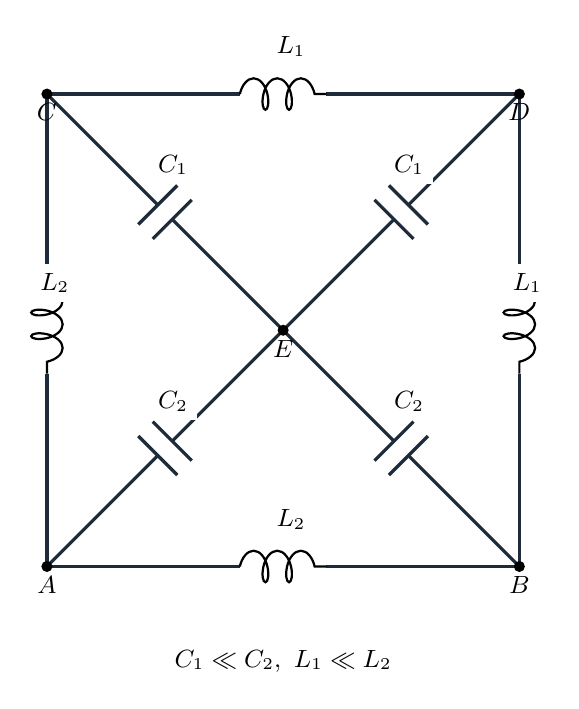
\begin{tikzpicture}[x=1cm,y=1cm,font=\small]
\begin{scope}[shift={(0.0,3.0)},rotate=0.0]
\draw[body](-3.0,0)--(-.55,0) (.55,0)--(3.0,0);\draw[thick,decorate,decoration={coil,aspect=.5,segment length=3mm,amplitude=2mm}](-.55,0)--(.55,0);\end{scope}
\node[fill=white]at(0.1,3.6){$L_1$};
\begin{scope}[shift={(0.0,-3.0)},rotate=0.0]
\draw[body](-3.0,0)--(-.55,0) (.55,0)--(3.0,0);\draw[thick,decorate,decoration={coil,aspect=.5,segment length=3mm,amplitude=2mm}](-.55,0)--(.55,0);\end{scope}
\node[fill=white]at(0.1,-2.4){$L_2$};
\begin{scope}[shift={(-3.0,0.0)},rotate=-90.0]
\draw[body](-3.0,0)--(-.55,0) (.55,0)--(3.0,0);\draw[thick,decorate,decoration={coil,aspect=.5,segment length=3mm,amplitude=2mm}](-.55,0)--(.55,0);\end{scope}
\node[fill=white]at(-2.9,0.6){$L_2$};
\begin{scope}[shift={(3.0,0.0)},rotate=-90.0]
\draw[body](-3.0,0)--(-.55,0) (.55,0)--(3.0,0);\draw[thick,decorate,decoration={coil,aspect=.5,segment length=3mm,amplitude=2mm}](-.55,0)--(.55,0);\end{scope}
\node[fill=white]at(3.1,0.6){$L_1$};
\begin{scope}[shift={(-1.5,1.5)},rotate=-45.0]
\draw[body](-2.1213203435596424,0)--(-.13,0) (.13,0)--(2.1213203435596424,0);\draw[body](-.13,-.35)--(-.13,.35) (.13,-.35)--(.13,.35);\end{scope}
\node[fill=white]at(-1.4,2.1){$C_1$};
\begin{scope}[shift={(1.5,1.5)},rotate=-135.0]
\draw[body](-2.1213203435596424,0)--(-.13,0) (.13,0)--(2.1213203435596424,0);\draw[body](-.13,-.35)--(-.13,.35) (.13,-.35)--(.13,.35);\end{scope}
\node[fill=white]at(1.6,2.1){$C_1$};
\begin{scope}[shift={(-1.5,-1.5)},rotate=45.0]
\draw[body](-2.1213203435596424,0)--(-.13,0) (.13,0)--(2.1213203435596424,0);\draw[body](-.13,-.35)--(-.13,.35) (.13,-.35)--(.13,.35);\end{scope}
\node[fill=white]at(-1.4,-0.9){$C_2$};
\begin{scope}[shift={(1.5,-1.5)},rotate=135.0]
\draw[body](-2.1213203435596424,0)--(-.13,0) (.13,0)--(2.1213203435596424,0);\draw[body](-.13,-.35)--(-.13,.35) (.13,-.35)--(.13,.35);\end{scope}
\node[fill=white]at(1.6,-0.9){$C_2$};
\fill (-3.000000,-3.000000) circle(2pt) node[below] {$A$};
\fill (3.000000,-3.000000) circle(2pt) node[below] {$B$};
\fill (-3.000000,3.000000) circle(2pt) node[below] {$C$};
\fill (3.000000,3.000000) circle(2pt) node[below] {$D$};
\fill (0.000000,0.000000) circle(2pt) node[below] {$E$};
\node at(0,-4.2){$C_1\ll C_2,\ L_1\ll L_2$};
\end{tikzpicture}

% 10 solution-05
\begin{tikzpicture}[x=1cm,y=1cm,font=\small]
\begin{scope}[shift={(0,1.8)}]\node at(0,2){高频};\draw[body](-3,-1)--(-3,1)--(-2,1);\draw[body](2,1)--(3,1)--(3,-1);\begin{scope}[shift={(-1.0,1.0)},rotate=0.0]
\draw[body](-1.0,0)--(-.13,0) (.13,0)--(1.0,0);\draw[body](-.13,-.35)--(-.13,.35) (.13,-.35)--(.13,.35);\end{scope}
\node[fill=white]at(-0.9,1.6){$C_1$};
\begin{scope}[shift={(1.0,1.0)},rotate=0.0]
\draw[body](-1.0,0)--(-.55,0) (.55,0)--(1.0,0);\draw[thick,decorate,decoration={coil,aspect=.5,segment length=3mm,amplitude=2mm}](-.55,0)--(.55,0);\end{scope}
\node[fill=white]at(1.1,1.6){$L_1$};
\begin{scope}[shift={(0.0,-1.0)},rotate=0.0]
\draw[body](-3.0,0)--(-.55,0) (.55,0)--(3.0,0);\draw[thick,decorate,decoration={coil,aspect=.5,segment length=3mm,amplitude=2mm}](-.55,0)--(.55,0);\end{scope}
\node[fill=white]at(0.1,-0.4){$L_1$};
\begin{scope}[shift={(0.0,0.0)},rotate=0.0]
\draw[body](-3.0,0)--(-.13,0) (.13,0)--(3.0,0);\draw[body](-.13,-.35)--(-.13,.35) (.13,-.35)--(.13,.35);\end{scope}
\node[fill=white]at(0.1,0.6){$C_1$};
\fill (-3.000000,0.000000) circle(2pt) node[left] {$E$};
\fill (3.000000,0.000000) circle(2pt) node[right] {$D$};
\end{scope}\begin{scope}[shift={(0,-3.2)}]\node at(0,2){低频};\draw[body](-3,-1)--(-3,1)--(-2,1);\draw[body](2,1)--(3,1)--(3,-1);\begin{scope}[shift={(-1.0,1.0)},rotate=0.0]
\draw[body](-1.0,0)--(-.13,0) (.13,0)--(1.0,0);\draw[body](-.13,-.35)--(-.13,.35) (.13,-.35)--(.13,.35);\end{scope}
\node[fill=white]at(-0.9,1.6){$C_2$};
\begin{scope}[shift={(1.0,1.0)},rotate=0.0]
\draw[body](-1.0,0)--(-.55,0) (.55,0)--(1.0,0);\draw[thick,decorate,decoration={coil,aspect=.5,segment length=3mm,amplitude=2mm}](-.55,0)--(.55,0);\end{scope}
\node[fill=white]at(1.1,1.6){$L_2/2$};
\begin{scope}[shift={(0.0,-1.0)},rotate=0.0]
\draw[body](-3.0,0)--(-.13,0) (.13,0)--(3.0,0);\draw[body](-.13,-.35)--(-.13,.35) (.13,-.35)--(.13,.35);\end{scope}
\node[fill=white]at(0.1,-0.4){$C_2$};
\fill (-3.000000,0.000000) circle(2pt) node[left] {$E$};
\fill (3.000000,0.000000) circle(2pt) node[right] {$D$};
\end{scope}\node[align=left,anchor=west]at(4,-.4){高频极点：$x^2-3x+1=0$\\低频极点：$y=4$};
\end{tikzpicture}

% 11 question-06
\begin{tikzpicture}[x=1cm,y=1cm,font=\small]
\draw[body,blue](0,0)ellipse(4 and 2.666667);\fill (-2.981424,0.000000) circle(2pt) node[below] {$O$};
\fill (0.000000,0.000000) circle(2pt) node[above] {$C$};
\fill (4.000000,0.000000) circle(2pt) node[right] {$e$};
\draw[vec](-2.9814239699997196,0)--(4,0)node[midway,above]{$r$};\draw[vec](4,0)--(4,1.2)node[right]{$v$};\draw[dim](-4,-3.2)--(4,-3.2)node[midway,below]{$2a$};\node at(0,3.4){O为焦点，C为椭圆中心};
\end{tikzpicture}

% 12 solution-06
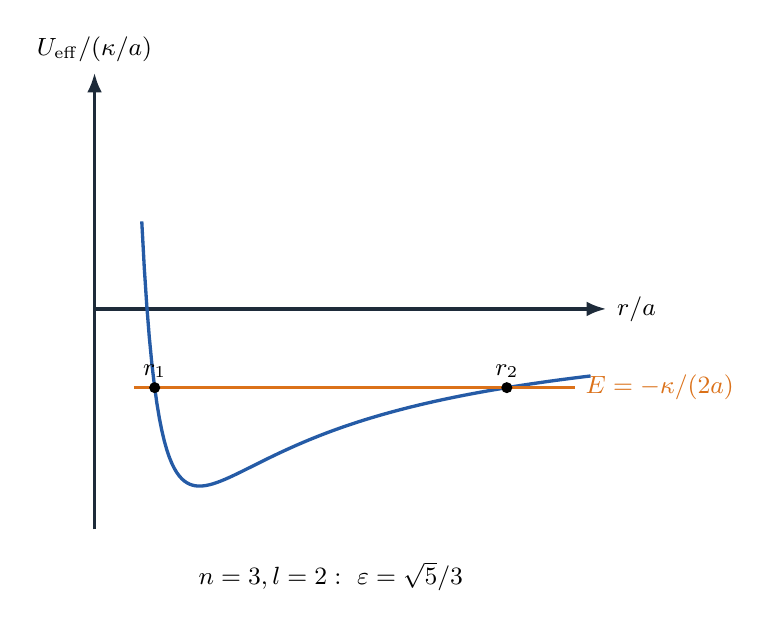
\begin{tikzpicture}[x=1cm,y=1cm,font=\small]
\draw[axis](0,0)--(6.5,0)node[right]{$r/a$};\draw[axis](0,-2.8)--(0,3)node[above]{$U_{\rm eff}/(\kappa/a)$};\draw[very thick,blue] plot coordinates {(0.600000,1.111111) (0.631844,0.523359) (0.663687,0.040585) (0.695531,-0.357994) (0.727374,-0.688460) (0.759218,-0.963386) (0.791061,-1.192705) (0.822905,-1.384330) (0.854749,-1.544620) (0.886592,-1.678723) (0.918436,-1.790837) (0.950279,-1.884405) (0.982123,-1.962270) (1.013966,-2.026789) (1.045810,-2.079932) (1.077654,-2.123347) (1.109497,-2.158422) (1.141341,-2.186332) (1.173184,-2.208073) (1.205028,-2.224492) (1.236872,-2.236315) (1.268715,-2.244163) (1.300559,-2.248571) (1.332402,-2.249999) (1.364246,-2.248845) (1.396089,-2.245454) (1.427933,-2.240125) (1.459777,-2.233119) (1.491620,-2.224663) (1.523464,-2.214955) (1.555307,-2.204170) (1.587151,-2.192457) (1.618994,-2.179952) (1.650838,-2.166771) (1.682682,-2.153017) (1.714525,-2.138780) (1.746369,-2.124141) (1.778212,-2.109169) (1.810056,-2.093926) (1.841899,-2.078468) (1.873743,-2.062842) (1.905587,-2.047091) (1.937430,-2.031252) (1.969274,-2.015359) (2.001117,-1.999441) (2.032961,-1.983524) (2.064804,-1.967630) (2.096648,-1.951779) (2.128492,-1.935988) (2.160335,-1.920274) (2.192179,-1.904649) (2.224022,-1.889125) (2.255866,-1.873713) (2.287709,-1.858421) (2.319553,-1.843256) (2.351397,-1.828226) (2.383240,-1.813335) (2.415084,-1.798589) (2.446927,-1.783991) (2.478771,-1.769545) (2.510615,-1.755253) (2.542458,-1.741118) (2.574302,-1.727140) (2.606145,-1.713322) (2.637989,-1.699664) (2.669832,-1.686165) (2.701676,-1.672827) (2.733520,-1.659650) (2.765363,-1.646632) (2.797207,-1.633773) (2.829050,-1.621073) (2.860894,-1.608531) (2.892737,-1.596144) (2.924581,-1.583913) (2.956425,-1.571836) (2.988268,-1.559911) (3.020112,-1.548137) (3.051955,-1.536512) (3.083799,-1.525034) (3.115642,-1.513702) (3.147486,-1.502515) (3.179330,-1.491469) (3.211173,-1.480565) (3.243017,-1.469798) (3.274860,-1.459169) (3.306704,-1.448674) (3.338547,-1.438312) (3.370391,-1.428082) (3.402235,-1.417980) (3.434078,-1.408006) (3.465922,-1.398158) (3.497765,-1.388433) (3.529609,-1.378830) (3.561453,-1.369347) (3.593296,-1.359981) (3.625140,-1.350733) (3.656983,-1.341598) (3.688827,-1.332577) (3.720670,-1.323666) (3.752514,-1.314865) (3.784358,-1.306171) (3.816201,-1.297583) (3.848045,-1.289099) (3.879888,-1.280718) (3.911732,-1.272438) (3.943575,-1.264257) (3.975419,-1.256174) (4.007263,-1.248187) (4.039106,-1.240295) (4.070950,-1.232496) (4.102793,-1.224789) (4.134637,-1.217172) (4.166480,-1.209644) (4.198324,-1.202203) (4.230168,-1.194849) (4.262011,-1.187579) (4.293855,-1.180393) (4.325698,-1.173289) (4.357542,-1.166266) (4.389385,-1.159322) (4.421229,-1.152457) (4.453073,-1.145668) (4.484916,-1.138956) (4.516760,-1.132318) (4.548603,-1.125754) (4.580447,-1.119263) (4.612291,-1.112842) (4.644134,-1.106492) (4.675978,-1.100211) (4.707821,-1.093999) (4.739665,-1.087853) (4.771508,-1.081773) (4.803352,-1.075759) (4.835196,-1.069808) (4.867039,-1.063921) (4.898883,-1.058096) (4.930726,-1.052332) (4.962570,-1.046628) (4.994413,-1.040984) (5.026257,-1.035399) (5.058101,-1.029871) (5.089944,-1.024400) (5.121788,-1.018985) (5.153631,-1.013625) (5.185475,-1.008319) (5.217318,-1.003068) (5.249162,-0.997869) (5.281006,-0.992722) (5.312849,-0.987626) (5.344693,-0.982581) (5.376536,-0.977586) (5.408380,-0.972640) (5.440223,-0.967743) (5.472067,-0.962893) (5.503911,-0.958090) (5.535754,-0.953334) (5.567598,-0.948624) (5.599441,-0.943959) (5.631285,-0.939338) (5.663128,-0.934762) (5.694972,-0.930229) (5.726816,-0.925738) (5.758659,-0.921290) (5.790503,-0.916883) (5.822346,-0.912517) (5.854190,-0.908192) (5.886034,-0.903907) (5.917877,-0.899661) (5.949721,-0.895454) (5.981564,-0.891285) (6.013408,-0.887154) (6.045251,-0.883061) (6.077095,-0.879004) (6.108939,-0.874984) (6.140782,-0.870999) (6.172626,-0.867050) (6.204469,-0.863136) (6.236313,-0.859257) (6.268156,-0.855412) (6.300000,-0.851600)};
\draw[very thick,orange](.5,-1)--(6.1,-1)node[right]{$E=-\kappa/(2a)$};\fill (0.763932,-1.000000) circle(2pt) node[above] {$r_1$};
\fill (5.236068,-1.000000) circle(2pt) node[above] {$r_2$};
\node at(3,-3.4){$n=3,l=2:\ \varepsilon=\sqrt5/3$};
\end{tikzpicture}

% 13 question-07
\begin{tikzpicture}[x=1cm,y=1cm,font=\small]
\draw[axis](-5,0)--(2,0);\draw[body](0,-1.8)--(0,1.8)node[above]{透镜};\draw[very thick,orange] plot coordinates {(-4.000000,0.000000) (-3.500000,0.866025) (-2.633975,0.366025) (-3.133975,-0.500000) (-4.000000,0.000000)};
\fill (-4.000000,0.000000) circle(2pt) node[above] {$D$};
\fill (-3.500000,0.866025) circle(2pt) node[above] {$A$};
\fill (-2.633975,0.366025) circle(2pt) node[above] {$B$};
\fill (-3.133975,-0.500000) circle(2pt) node[above] {$C$};
\fill (-2.000000,0.000000) circle(2pt) node[below] {$F$};
\fill (2.000000,0.000000) circle(2pt) node[below] {$F'$};
\draw[dim](-4,-1.1)--(0,-1.1)node[midway,below]{$2f$};\draw[guide](-4,0)--(-3.2,0);\draw(-3.4,0)arc(0:-30:.6)node[midway,left,xshift=-3mm]{$30^\circ$};
\end{tikzpicture}

% 14 solution-07
\begin{tikzpicture}[x=1cm,y=1cm,font=\small]
\draw[axis](-.2,0)--(7.2,0)node[right]{$x\prime/f$};\draw[axis](0,1.8)--(0,-2.3)node[below]{$y\prime/f$（向下）};\draw[very thick,blue] plot coordinates {(2.000000,-0.000000) (2.666667,-1.154701) (6.309401,-1.154701) (3.527416,0.881854) (2.000000,-0.000000)};
\fill (2.000000,-0.000000) circle(2pt) node[below] {$D'$};
\fill (2.666667,-1.154701) circle(2pt) node[below] {$A'$};
\fill (6.309401,-1.154701) circle(2pt) node[below] {$B'$};
\fill (3.527416,0.881854) circle(2pt) node[below] {$C'$};
\node[align=left]at(4,2.5){$X\prime=1/X,\ Y\prime=Y/X$\\$S=(84+34\sqrt3)f^2/117$};
\end{tikzpicture}

% 15 question-08
\begin{tikzpicture}[
  x={(.72cm,-.30cm)},y={(1cm,0cm)},z={(0cm,1cm)},scale=.83
]
  % 两根长直导线位于半透明的 yz 平面内。
  \fill[ink!5]
    (0,-4.75,-2.45)--(0,4.75,-2.45)--(0,4.75,3.45)--(0,-4.75,3.45)--cycle;
  \draw[draw=ink!30,thin]
    (0,-4.75,-2.45)--(0,4.75,-2.45)--(0,4.75,3.45)--(0,-4.75,3.45)--cycle;
  \node[ink!65,anchor=south west,fill=white,inner sep=1.5pt]
    at (0,-4.65,3.45) {$yz$ 平面};
  \draw[body,line width=1.35pt] (0,-4,-2.25)--(0,-4,3.2);
  \draw[body,line width=1.35pt] (0,4,-2.25)--(0,4,3.2);
  \draw[current] (0,-4,-1.8)--(0,-4,2.55) node[left=2pt] {$I$};
  \draw[current] (0,4,2.55)--(0,4,-1.8) node[right=2pt] {$I$};
  \draw[dim] (0,-4,3.75)--(0,4,3.75)
    node[pos=.38,above,fill=white,inner sep=2pt] {$2a$};

  % 线框的水平边沿 xy 平面内的倾斜方向，竖边始终平行于 z 轴。
  \coordinate (P1) at (-1.75,-2.20,-1.45);
  \coordinate (P2) at ( 1.75, 2.20,-1.45);
  \coordinate (P3) at ( 1.75, 2.20, 1.70);
  \coordinate (P4) at (-1.75,-2.20, 1.70);
  \fill[blue!13,opacity=.72] (P1)--(P2)--(P3)--(P4)--cycle;
  \draw[very thick,blue] (P1)--(P2)--(P3)--(P4)--cycle;
  \draw[current,orange] (P1)--(P4);
  \draw[current,orange] (P3)--(P2);
  \draw[dim] (-1.75,-2.20,2.05)--(1.75,2.20,2.05)
    node[midway,above left,fill=white,inner sep=1pt] {$2b$};
  \draw[dim] (2.15,1.85,-1.45)--(2.15,1.85,1.70)
    node[midway,right] {$d$};

  % 转轴和俯视角：角 phi 是线框平面与 yz 平面的夹角。
  \draw[axis] (0,0,-2.55)--(0,0,3.95) node[above] {$z$};
  \coordinate (Ophi) at (0,0,-2.35);
  \coordinate (Yphi) at (0,3.05,-2.35);
  \coordinate (Uphi) at (1.75,2.20,-2.35);
  \draw[guide] (Ophi)--(Yphi);
  \draw[guide] (Ophi)--(Uphi);
  \pic[draw=ink,"$\phi$",angle radius=8mm,angle eccentricity=1.25]
    {angle=Uphi--Ophi--Yphi};
  \node[below right] at (Yphi) {$y$};
  \draw[-{Latex[length=2mm]},draw=ink!55,thick]
    (Ophi)--(1.35,0,-2.35) node[below right] {$x$};
  \node[blue!70!black,anchor=north] at (0,0,-3.15)
    {矩形线框绕中心 $z$ 轴转动};
\end{tikzpicture}

% 16 solution-08
\begin{tikzpicture}[x=1cm,y=1cm,font=\small]

\draw[axis](-2.2,0)--(3.2,0)node[right]{$x$};\draw[axis](0,-4.7)--(0,4.7)node[above]{$y$};
\node at(0,4){$\otimes$};\node[right]at(.3,4){$y=+a,-I\hat z$};\node at(0,-4){$\odot$};\node[right]at(.3,-4){$y=-a,+I\hat z$};
\draw[body,blue](-1.5,-2)--(1.5,2);\node at(1.5,2){$\otimes$};\node at(-1.5,-2){$\odot$};
\draw[dim](0,0)--(1.5,2)node[midway,right]{$b$};\draw[guide](0,4)--(1.5,2)node[midway,right]{$r_1$};\draw[guide](0,-4)--(1.5,2)node[midway,right]{$r_2$};
\draw(0,1)arc(90:53.13:1)node[midway,above]{$\phi$};
\node[align=left,anchor=west]at(4,0){顶视图：$\boldsymbol u=(\sin\phi,\cos\phi)$\\$\phi$为顺时针角\\$Q_\phi=-M,\ \tau_z=+M$\\$r_{1,2}^2=a^2+b^2\mp2ab\cos\phi$};
\end{tikzpicture}
\end{document}
